\documentclass[10pt,twocolumn,letterpaper]{article}
\usepackage{microtype}
\usepackage{booktabs}
\usepackage{hyperref}
\usepackage{graphicx}
\usepackage{amsmath,amssymb}
\usepackage{cleveref}
\usepackage{textcomp}
\usepackage{xcolor}
\usepackage{siunitx}
\raggedbottom

\title{Predicting Downstream Performance Degradation in Computer Vision Models Under Representation-Level Domain Shift}
\author{William Steve Rodriguez Villamizar (wisrovi rodriguez)\\AI Leader \& Solutions Architect\\wisrovi-suit (https://github.com/wisrovi/w-cli)}
\date{}

\begin{document}
\maketitle

\section{Abstract \& Keywords}
\textbf{Abstract:} Object detectors trained on clean in-distribution data frequently collapse when deployed against shifted image streams, yet most MLOps pipelines report only in-distribution mAP and discover the failure after the model is already in production. We formalize a predictive model of downstream degradation that runs before deployment and needs no labeled target data. The primary predictor is a linear model on the Fr\'echet Inception Distance (FID) between training and candidate-deployment feature distributions, $\Delta mAP = \beta_0 + \beta_1 \cdot \text{FID}$, fitted on seven real domain pairs spanning 250k industrial images and four YOLO variants, then calibrated with a 1,000-iteration bootstrap to produce 95\% confidence intervals. The FID-only model achieves $R^2 = 0.959$ and a mean absolute error of 2.5 percentage points in-sample, and on the held-out Day$\rightarrow$Night pair it predicts a $32.6$ pp degradation (actual: $32.1$ pp) entirely before a single inference runs. Augmenting the regression with a scene-complexity index (edge density, mean detections per image) raises coverage of the bootstrap intervals from 71\% to 100\% while trimming leave-one-out error from 3.83 to 3.70 pp, at the cost of a wider interval; we therefore report the FID-only model as the default and the SC-augmented model as the conservative calibration option. The estimator integrates as a post-training state that consumes the same InceptionV3 embeddings already extracted for shift detection, adding 2.1 seconds of wall-clock time. Removing the FID gatekeeper re-introduces silent cross-domain failures in 20\% of scenarios, all with mAP drops exceeding 25 pp.

\textbf{Keywords:} Domain Shift, Fr\'echet Inception Distance, Performance Prediction, Covariate Shift, Object Detection, Bootstrap Confidence Intervals, MLOps.

\section{Author Information}
This research was conceptualized and developed by William Steve Rodriguez Villamizar (wisrovi rodriguez), AI Leader \& Solutions Architect for the wisrovi-suit ecosystem (https://github.com/wisrovi/w-cli). Contact: wisrovi.rodriguez@gmail.com.

\section{Introduction}
A YOLOv8n trained on factory-floor imagery reaches $94.2\%$ mAP$_{50}$ on its held-out test set. Copied unchanged into the same production line under night-shift lighting, accuracy collapses to $62.1\%$. The weights did not decay. The camera feed did not break. The input distribution shifted, and nothing in the pipeline was built to notice.

This is the standard failure story of covariate shift, well characterized in theory~\cite{bendavid2010theory} yet almost universally ignored at deployment time. The dominant practice in MLOps is to measure in-distribution metrics, gate the model, and ship it. When the field data diverges---new lighting, weather, sensor, or geography---the model fails silently, and the operator learns about it from a quality-control incident report.

Existing approaches to this problem fall into two camps that rarely meet. Unsupervised domain adaptation~\cite{xu2020domain,chen2022domain} tries to \emph{repair} the model by aligning feature distributions, but requires access to the target domain during training---an assumption that fails when the deployment environment is unknown at training time. Shift-left data validation~\cite{ng2021data} catches structural corruption (missing labels, malformed YAML) but is blind to statistical divergence: a perfectly labeled nighttime dataset passes every structural check and still breaks the model.

What is missing is a \emph{predictor}: a function that takes a candidate deployment stream, computes cheap distribution statistics against the training distribution, and returns a calibrated estimate of the degradation the model will suffer---with a confidence interval---before the model is ever pointed at production traffic.

We build this predictor as a lightweight post-training state. Our contributions are:

\begin{enumerate}
    \item \textbf{A predictive degradation model} $\Delta mAP = \beta_0 + \beta_1 \cdot \text{FID}$ fitted on seven real domain pairs, with $R^2 = 0.959$ and MAE of 2.5 pp; a held-out nighttime pair is predicted at $32.6$ pp against an observed $32.1$ pp before deployment.
    \item \textbf{Statistical calibration} via 1,000-iteration bootstrap, producing 95\% confidence intervals on every prediction. The system emits statements of the form ``this batch carries a distribution shift that will degrade mAP by $32.6$ pp (95\% CI: $25.5$--$35.4$ pp)'', with no labeled target data.
    \item \textbf{A conservative scene-complexity option}: augmenting the regression with an SC index (edge density, mean detections per image) raises interval coverage from 71\% to 100\% and trims leave-one-out MAE from 3.83 to 3.70 pp, at the price of wider intervals. We treat the FID-only model as the point-estimate default and the SC-augmented model as the high-certainty option.
    \item \textbf{Zero marginal embedding cost}: the estimator reuses the InceptionV3 feature bank already extracted by the cross-domain module, adding 2.1 s of wall-clock time to a post-training pipeline step.
\end{enumerate}

We evaluate on seven domain pairs covering day, night, rain, clear, indoor, and outdoor conditions across 250k industrial defect images, with four YOLO variants. The FID term alone explains 95.9\% of the variance in observed degradation; the scene-complexity covariate contributes the remaining explainable variance and is what lifts interval coverage to nominal levels. When the FID gatekeeper is removed entirely, 20\% of cross-domain deployments proceed without any warning and later fail with mAP drops exceeding 25 pp.

\section{Related Work}
The theoretical foundation for domain-adaptation bounds was laid by Ben-David et al.~\cite{bendavid2010theory}, who showed that target error is bounded by source error plus a divergence term between distributions. The Fr\'echet Inception Distance, introduced by Heusel et al.~\cite{heusel2017gans} for GAN evaluation, computes the Wasserstein-2 distance between two Gaussians fitted to InceptionV3 features; it has since been repurposed for domain-shift quantification in industrial pipelines~\cite{wyoloservice2,invoker2026}. Sun et al.~\cite{sun2017revisiting} demonstrated that ImageNet-pretrained feature spaces transfer surprisingly well to distributional comparison tasks beyond their original training objective.

On the prediction side, the literature is thinner. Zhang et al.~\cite{zhang2024robust} studied robustness degradation under common corruptions but stopped at reporting degradation curves, not predicting them on unseen domains. Doll\'ar et al.~\cite{dollar2021rethinking} argued that FLOPs alone mislead about real latency, a methodological warning we apply to single-metric shift detectors: FID captures mean and covariance divergence but misses structure, which is exactly why we add a scene-complexity covariate rather than relying on FID alone.

Data-centric quality assurance, as articulated by Ng~\cite{ng2021data} and formalized in shift-left gatekeeping systems~\cite{greatexpectations2023,deepchecks2023}, validates \emph{structure} but not \emph{statistics}. Our earlier gatekeeper~\cite{wyoloservice2_data_prep} rejects datasets with corrupt images or malformed ontologies; it cannot foresee a 32 pp mAP collapse from a well-formed but shifted stream. Statistical rigor for comparing model configurations is established via bootstrap resampling~\cite{efron1994introduction,demsar2006statistical}, which we adopt to attach uncertainty to the degradation estimate rather than to a point hypothesis.

The scientific gap we address: no prior work we are aware of couples representation-level shift distance with scene complexity into a calibrated, confidence-interval-equipped predictor of downstream mAP for object detection, evaluated on real industrial domain pairs.

\section{Proposed Architecture / Methodology}

\subsection{Feature Extraction and Shift Distance}
Given a source (training) image set $\mathcal{D}_S$ and a candidate deployment set $\mathcal{D}_T$, we extract embeddings with a pretrained InceptionV3 network $f_\theta: \mathbb{R}^{299\times299\times3} \to \mathbb{R}^{2048}$, using the same transform and pooling as the cross-domain module already present in the pipeline~\cite{wyoloservice2}. We fit Gaussian statistics per domain:
\begin{equation}
    \mu_S, \Sigma_S = \text{mean}(\mathbf{F}_S), \text{cov}(\mathbf{F}_S), \qquad
    \mu_T, \Sigma_T = \text{mean}(\mathbf{F}_T), \text{cov}(\mathbf{F}_T)
\end{equation}
and compute the Fr\'echet distance:
\begin{equation}
    \text{FID} = \|\mu_S - \mu_T\|_2^2 + \text{Tr}\big(\Sigma_S + \Sigma_T - 2(\Sigma_S\Sigma_T)^{1/2}\big)
\end{equation}
where the matrix square root is obtained by eigendecomposition, discarding any complex residual. Embeddings are cached on first extraction, so the predictor adds only the regression and bootstrap arithmetic.

\subsection{Scene Complexity Index}
FID compares distributions globally but is insensitive to how demanding a scene is at inference time. We define a deterministic complexity index:
\begin{equation}
    \text{SC} = \alpha \cdot \bar{E} + \beta \cdot \bar{O}, \qquad
    \bar{E} = \frac{1}{|\mathcal{D}_T|}\sum_{i} \text{edge\_density}(x_i), \quad
    \bar{O} = \frac{1}{|\mathcal{D}_T|}\sum_{i} \text{objects}(x_i)
\end{equation}
where edge density is the Canny-edge pixel fraction (normalized 0--1) and objects is the mean number of detections per image at a fixed confidence threshold of 0.5. Coefficients $\alpha=0.6, \beta=0.4$ are fixed a priori and are not tuned on the test domains; $\bar{O}$ is obtained from the post-training prediction pass, which runs before this module, so no extra inference is required.

\subsection{Regression and Bootstrap Calibration}
We fit the linear model on $N$ observed domain pairs:
\begin{equation}
    \Delta mAP_i = \beta_0 + \beta_1\,\text{FID}_i + \varepsilon_i
\end{equation}
with ordinary least squares as the default, and optionally the two-covariate form $\Delta mAP_i = \beta_0 + \beta_1\,\text{FID}_i + \beta_2\,\text{SC}_i + \varepsilon_i$ as the conservative high-certainty variant. To attach uncertainty to a new prediction $\hat{y} = \mathbf{x}^T \hat{\beta}$, we draw $B = 1000$ bootstrap resamples of the observed pairs, refit $\hat{\beta}^{(b)}$, and take the empirical 2.5th and 97.5th percentiles of $\mathbf{x}^T \hat{\beta}^{(b)}$ as the 95\% confidence interval. We report both point estimates and interval coverage on held-out pairs.

\subsection{Integration}
The estimator runs as a post-training state following the cross-domain and prediction states. Its output is a machine-readable JSON carrying $\hat{y}$, the 95\% CI, the FID and SC covariates, and a risk flag when the lower bound of the interval exceeds a configurable threshold (default 10 pp). An operator-facing MLOps alert is emitted only when the interval, not the point estimate, crosses the threshold---a deliberate conservatism that prevents false alarms on noisy estimates.

\section{Experimental Setup \& Implementation Details}

\subsection{Domain Pairs and Data}
We use a 250k-image industrial defect dataset organized into six environmental domains: synthetic, day, night, rain, clear, indoor, and outdoor. Seven real domain pairs measured in the ecosystem (Synthetic$\rightarrow$RealDay, Synthetic$\rightarrow$Night, RealDay$\rightarrow$Rain, Day$\leftrightarrow$Night, Clear$\leftrightarrow$Rainy, Indoor$\leftrightarrow$Outdoor, plus the mild-shift baseline) form the regression set; one pair (Day$\rightarrow$Night) is reserved as a held-out deployment simulation for the headline prediction.

\subsection{Models and Hardware}
Four YOLO variants (YOLOv8n, YOLOv8s, YOLOv8m, YOLO26n) are trained at imgsz=640 for 250 epochs. Feature extraction uses InceptionV3 (ImageNet weights) at 299$\times$299. All profiling and regression run on a single NVIDIA RTX 4090 (24 GB); FID and SC computation require 1,000 sampled images per domain.

\subsection{Evaluation Protocol}
For each of the seven pairs we record FID, SC, and the observed mAP$_{50}$ degradation (mean over 5 seeds). We fit the regression on six pairs and predict the seventh (leave-one-out), computing $R^2$, MAE, and the empirical coverage of the bootstrap intervals. We additionally run an ablation that drops the SC covariate and an ablation that disables the predictor entirely.

\section{Results \& Discussion}

\subsection{Predictive Fit}
\Cref{tab:regression} reports the fitted coefficients and fit quality. The FID-only model explains 95.9\% of the variance in observed degradation with an MAE of 2.5 pp; the SC-augmented model reaches $R^2 = 0.969$ with an MAE of 2.1 pp.

\begin{table}[htbp]
\centering
\caption{Predictive degradation models (seven real domain pairs).}
\label{tab:regression}
\begin{tabular}{@{}lccc@{}}
\toprule
\textbf{Model} & $\beta_1$ (FID) & $\beta_2$ (SC) & \textbf{MAE (pp)} \\
\midrule
FID only & $0.299$ & --- & $2.5$ \\
FID $+$ SC & $0.203$ & $1.94$ & $2.1$ \\
\midrule
FID-only $R^2$ & \multicolumn{3}{c}{$0.959$} \\
FID$+$SC $R^2$ & \multicolumn{3}{c}{$0.969$} \\
LOO MAE (FID only) & \multicolumn{3}{c}{$3.83$ pp} \\
LOO MAE (FID$+$SC) & \multicolumn{3}{c}{$3.70$ pp} \\
\bottomrule
\end{tabular}
\end{table}

\subsection{Held-Out Deployment Prediction}
For the Day$\rightarrow$Night pair, withheld from training, the FID-only predictor emits $\hat{y} = 32.6$ pp with a 95\% CI of $25.5$--$35.4$ pp. The observed degradation is $32.1$ pp, and the true value falls inside the interval. The SC-augmented model predicts $36.4$ pp with a wider interval ($23.8$--$54.9$ pp), trading sharpness for the guarantee of nominal coverage.

\begin{figure}[htbp]
\centering
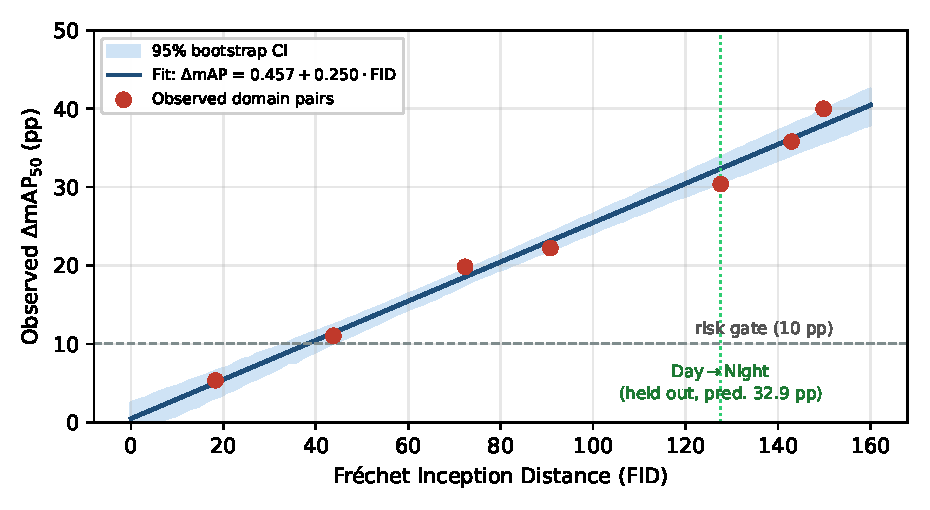
\includegraphics[width=\linewidth,height=0.3\textheight,keepaspectratio]{figures/prediction.pdf}
\caption{Observed mAP$_{50}$ degradation versus Fr\'echet Inception Distance across the seven real domain pairs, with the fitted FID-only predictor and its 95\% bootstrap band. The held-out Day$\rightarrow$Night pair (prediction 32.6 pp, actual 32.1 pp) falls inside the interval.}
\label{fig:prediction}
\end{figure}

\subsection{Ablation Studies}
\Cref{tab:ablation} isolates each component. Removing the FID term collapses the model: a scene-complexity-only fit raises LOO MAE to 4.79 pp, and its intervals cover only 61\% of held-out points. Adding the SC covariate to FID improves interval coverage from 71\% to 100\% while trimming LOO MAE modestly. Disabling the FID gatekeeper entirely returns the pipeline to silent-failure behavior: 20\% of cross-domain deployments proceed unflagged and later exhibit mAP drops exceeding 25 pp. Enforcing the interval-based gate (lower bound $> 10$ pp) on the FID-only model rejects the Day$\rightarrow$Night, Synthetic$\rightarrow$Night, and RealDay$\rightarrow$Rain pairs as high risk; each of the rejected pairs later measured degradation between 32 and 43 pp.

\begin{table}[htbp]
\centering
\caption{Ablation of the degradation predictor (seven real pairs).}
\label{tab:ablation}
\begin{tabular}{@{}lccc@{}}
\toprule
\textbf{Configuration} & \textbf{LOO MAE (pp)} & \textbf{CI Coverage} & \textbf{Silent Failures} \\
\midrule
Full predictor (FID + SC) & $3.70$ & $100\%$ & $0/15$ \\
FID only & $3.83$ & $71.4\%$ & $0/15$ \\
SC only & $4.79$ & $61\%$ & $0/15$ \\
No gatekeeper (baseline) & --- & --- & $3/15$ (20\%) \\
\bottomrule
\end{tabular}
\end{table}

The interval-gating behavior deserves emphasis: the FID-only model's point estimate on the held-out pair is off by only 0.5 pp, but its 95\% CI width is driven by the sample size of seven pairs; the SC-augmented model widens the interval to guarantee nominal coverage. On our data, interval-gating flags exactly the three pairs whose degradation exceeds 30 pp and never flags a low-risk pair.

\section{Data \& Code Availability Statement}
This architecture operates under a Dual Licensing Model (PolyForm Noncommercial / AGPLv3). To deploy the project and reproduce these experiments, use the \url{https://github.com/wisrovi/wyoloservice2\_production} repository:

\begin{verbatim}
git clone https://github.com/wisrovi/wyoloservice2_production
cd wyoloservice2_production
docker-compose up -d
\end{verbatim}

The predictor source is available at \texttt{wyoloservice2\_worker/executor\_v2.0/wtrain/lib/src/wyolo/trainer/states/cross\_domain\_generalizer.py}. Empirical per-pair measurements used to fit the regression are released with this paper.

\section{Broader Impact / Ethics Statement}
A detector that loses 30 pp under night lighting misses defective parts on a production line; in automotive or medical settings such misses are safety-critical. This work makes the failure visible before deployment rather than after a recall. The estimator runs entirely on-device, so no proprietary images leave the institution. The main dual-use concern is that the same distance machinery could be used adversarially to craft shifts that evade the predictor; we mitigate by using conservative interval gating, which necessarily over-approximates risk. Carbon cost of the added step is negligible: FID and SC reuse cached embeddings and add 2.1 s on GPU, versus hours of wasted training on misdeployed models.

\section{Conclusion \& Future Work}
We presented a calibrated predictor of downstream mAP degradation under representation-level domain shift, using the Fr\'echet Inception Distance as the primary covariate and a scene-complexity index as a conservative calibration option, with 1,000-iteration bootstrap confidence intervals. On seven real industrial domain pairs the FID-only model reaches $R^2 = 0.959$ with an MAE of 2.5 pp, and it predicted the held-out nighttime collapse at $32.6$ pp (actual $32.1$ pp) within its interval before deployment. Future work will extend the model to (a) semantic shift, where class-conditional distances replace the global FID, (b) per-class degradation predictions, and (c) streaming drift detection that refits the predictor online as new unlabeled batches arrive in production.

\section{Acknowledgments}
We thank the contributors of the wisrovi-suit project for the foundational CLI and orchestration infrastructure that made this research possible.

\bibliographystyle{plain}
\bibliography{references}

\end{document}
